\begin{frame}[allowframebreaks]{Laufzeitanalyse}
    \label{frame:runtime_analysis}
    %Diskrete, direkte Convolution
    \begin{figure}
        \centering
        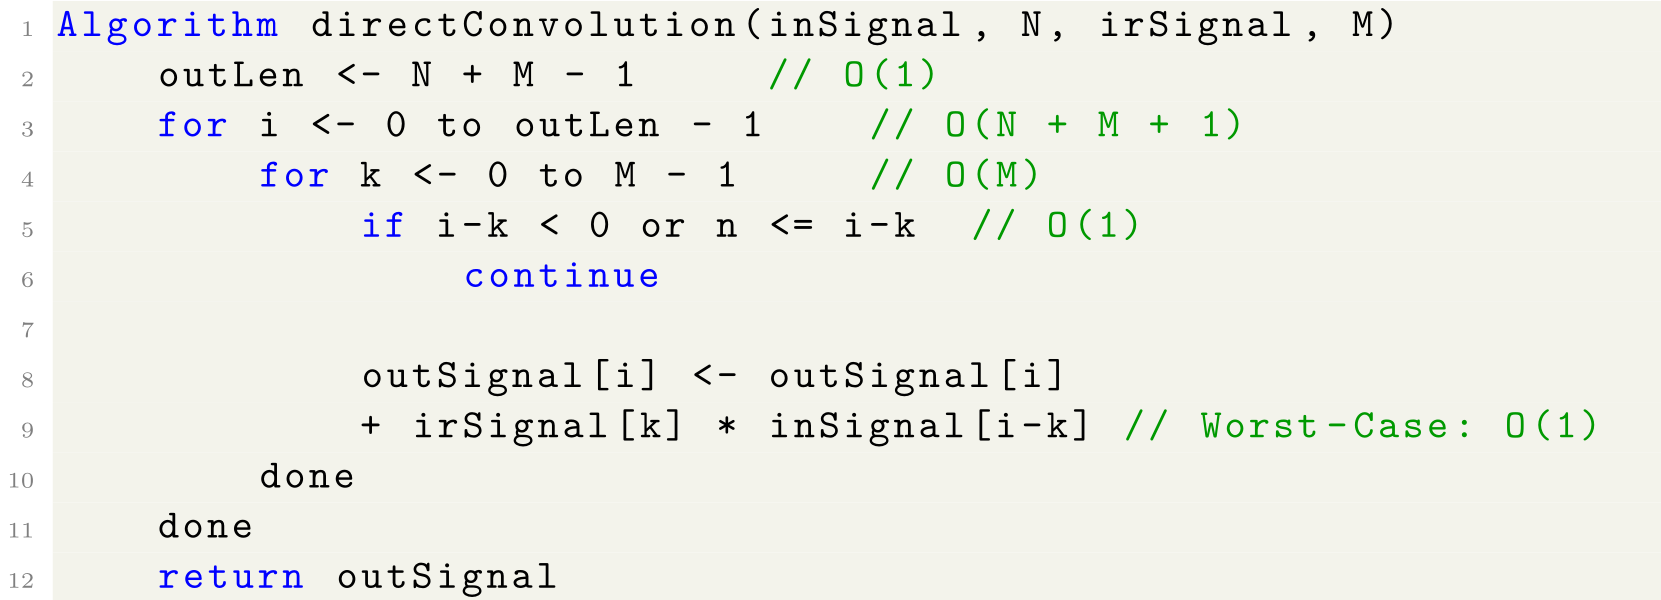
\includegraphics[width=0.9\textwidth]{Graphics/pseudocode_diskrete_convolution.png}
        \caption{Pseudocode: Implementierung der diskreten Convolution}
    \end{figure}
    \framebreak
    \begin{itemize}
        \item Worst-Case Laufzeitklasse:
    \end{itemize}
    \begin{equation}
        \mathcal{O}(1 + (N + M - 1) \cdot (M + 2)) = \mathcal{O}(M^2 + NM - M + 2N - 1)
    \end{equation}
    \begin{itemize}
        \item ... vereinfacht sich lt. Polynomregel zu:
    \end{itemize}
    \begin{equation}
        \mathcal{O}(M^2 + NM)
    \end{equation}
    \begin{itemize}
        \item ... es gilt aber
    \end{itemize}
    \begin{equation}
        N \gg M \implies N \cdot M > M^2
    \end{equation}
    \begin{itemize}
        \item ... woraus folgt: $\mathcal{O}(N \cdot M)$
        \label{fig: runtime_direct_convolution}

        \framebreak

        \item Umwandlung eines Signals in Zeitdomäne in Frequenzdomäne mithilfe der \textit{Fourier Transformation}:
        \begin{equation}
            X[m] = \sum_{n = 0}^{N - 1}x[n] \cdot e^{\frac{-i2\pi \cdot nm}{N}}
        \end{equation}
    \end{itemize}

    %FFT-Convolution

    \begin{figure}
        \centering
        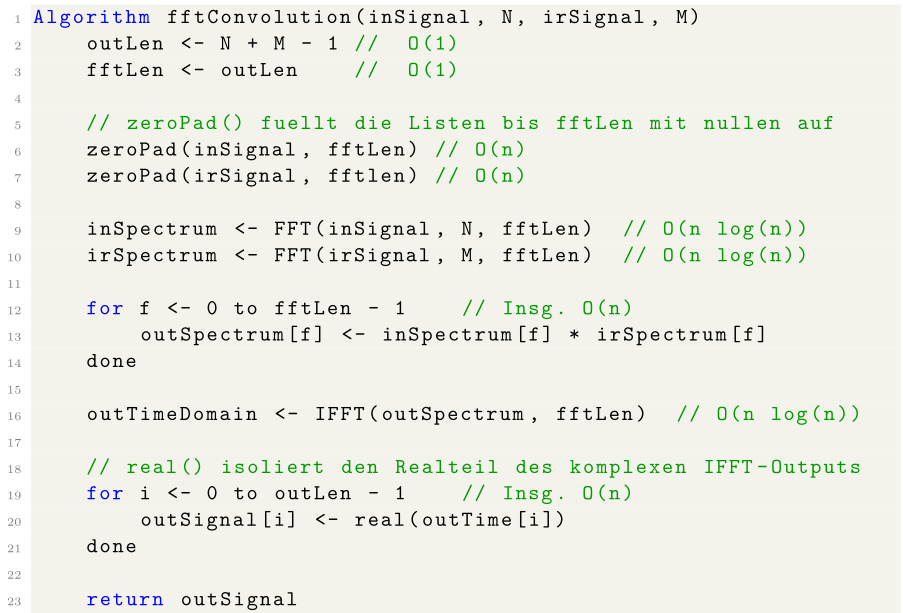
\includegraphics[width=0.6\textwidth]{Graphics/pseudocode_fft_convolution.png}
        \caption{Pseudocode: Implementierung der Convolution mithilfe der
        \textit{Fast Fourier Transformation}}
    \end{figure}
    \begin{itemize}
        \item Laufzeit:
    \end{itemize}
    \begin{equation}
        \mathcal{O}(3(N \cdot \log(N)) + 4N + 2) \in \mathcal{O}(N \cdot \log(N))
    \end{equation}
\end{frame}